\documentclass[border=4pt]{standalone}
% Preámbulo común de las figuras. Cada figura es un documento standalone
% que se compila a SVG con scripts/build_figures.sh
\usepackage[utf8]{inputenc}
\usepackage{amsmath}
\usepackage{tikz}
\usepackage[american, siunitx]{circuitikz}
\usetikzlibrary{arrows.meta,calc,decorations.pathmorphing,patterns}
\tikzset{
  >={Stealth[length=2.2mm]},
  eje/.style={->, thin},
  hilo/.style={thick},
}
% Paleta común: tonos medios legibles sobre fondo claro
\definecolor{azul}{RGB}{31,94,168}
\definecolor{rojo}{RGB}{192,57,43}
\definecolor{verde}{RGB}{39,128,73}
\definecolor{naranja}{RGB}{211,120,30}
\definecolor{morado}{RGB}{125,60,152}

\begin{document}
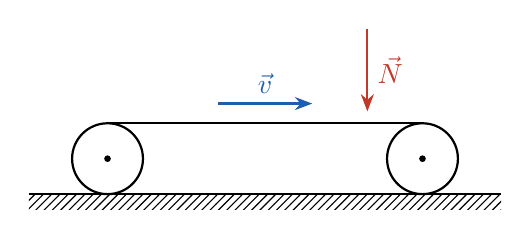
\begin{tikzpicture}[scale=1.0]
  \fill[pattern=north east lines] (-1.0,-0.2) rectangle (5.0,0);
  \draw[thick] (-1.0,0) -- (5.0,0);
  \draw[thick] (0,0.45) circle (0.45);
  \draw[thick] (4,0.45) circle (0.45);
  \fill (0,0.45) circle (1.2pt); \fill (4,0.45) circle (1.2pt);
  \draw[thick] (0,0.9) -- (4,0.9);
  \draw[thick] (0,0.0) -- (4,0.0);
  \draw[->, thick, azul] (1.4,1.15) -- (2.6,1.15) node[midway, above]{$\vec{v}$};
  \draw[->, thick, rojo] (3.3,2.1) -- (3.3,1.05) node[midway, right]{$\vec{N}$};
\end{tikzpicture}
\end{document}
